\documentclass[11pt,a4paper]{article}

\usepackage{mynotes}

\usepackage{dcolumn}
\usepackage{multirow}

\title{A regional scale assessment of the biodiversity - ecosystem function relationship in southern African woodlands}
\author{John L. Godlee}
\date{}

\newcommand{\nplots}{1749}
\newcommand{\nplotspcoa}{1859}


\begin{document}

\maketitle
\tableofcontents

\section{Introduction}

A number of studies have shown relationships between biodiversity and ecosystem functionality \citep{Review}. Ecosystem functions can be defined in broad terms as rate processes and properties which describe the degree of biotic activity within an ecosystem \citep{Jax2005}. This includes basic processes of primary production such as gross primary productivity and atmospheric nitrogen fixation, but can be extended to indirect aggregate measures of function such as resistance of productivity to disturbance \citep{}. Ecosystem functionality may also include static ecosystem properties such as forest canopy complexity and trophic complexity, which in turn influence ecosystem processes. The strength and direction of these observed Biodiversity - Ecosystem Function Relationships (BEFRs) varies depending on the ecosystem being studied \citep{}, the ecosystem function(s) of interest \citep{}, and the inclusion of environmental covariates in statistical models \citep{}, but there appears to be a generalisable positive correlation between biodiversity and ecosystem functionality \citep{Liang2016}. Over the past decade, many observational studies of the BEFR have been conducted, mostly in tropical and temperate forests, and grasslands \citep{Chen2011}. These studies support previous findings from small scale experimental studies which began in earnest during the 1990s as concern grew over the global loss of biodiversity \citep{Tilman1994, Tilman2014}.

The representation of dry tropical ecosystems in the BEFR literature is poor compared to other ecosystems. \citet{Clarke2017} conducted a meta-analysis of 182 published BEFR studies, finding that only 13\% were conducted in the tropics, with 42\% of those being conducted in the highly endemic wet tropical forests of Costa Rica. In wet tropical forests, much of the observed effect of biodiversity on ecosystem function has been attributed to niche complementarity \citep{}, whereby competition between individuals is reduced due to them occupying different niche space, allowing diverse species assemblages to take greater advantage of natural resources \citep{}. In the dry tropics however, low precipitation, high seasonality of rainfall and temperature, and high levels of disturbance from fire and herbivory mean that niche complementarity and competition may not play as much of a role in the relationship between biodiversity and ecosystem function. Instead, stress tolerance and productivity of abundant species (selection effects) may be the predominant forces which influence ecosystem functionality \citep{}. Similarly, more diverse species assemblages may lead to facilitation effects between certain species combinations in environments which are more hostile to growth \citep{}.

In the seasonally dry woodlands of southern Africa, human actions are driving rapid changes in biodiversity. This has in turn raised interest in how biodiversity influences ecosystem function in these ecosystems \citep{}. Resource extraction by humans directly influences biodiversity via selective tree-felling for timber, charcoal making, non-timber forest products and through land use change to agriculture \citep{Ryan2016}. Climate change is also indirectly affecting the biodiversity of southern African woodlands, altering temperature and precipitation, and affecting climate seasonality \citep{}. Savannas and sparse woodlands are the dominant vegetation type across the southern African region, spanning >4 million km\textsuperscript{2} \citep{Ryan2016}. The carbon stored in these woodlands is comparable to that found in the wet forests of the Congo basin and are of global importance to the carbon cycle. Climatic conditions and biogeography vary across southern African woodlands, resulting in a diverse range of woodland tree species assemblages, which retain the common features of an open tree canopy and an understorey generally dominated by C4 grass species \citep{Frost1996}. Southern African woodlands are highly diverse, thought to harbour \textapprox{}8500 plant species of which there are >300 tree species \citep{Frost1996}. These ecosystems have been identified by previous studies as a priority for conservation efforts \citep{Brooks2006, Mittermeier2003, Frost1996}. Many conservation projects in the region currently aim to conserve biodiversity and woody biomass stocks simultaneously under the directive of the United Nations REDD+ programme or the similar Forest Carbon Partnership Facility (FCPF) \citep{Hinsley2015}. A small number of academic studies in southern African woodlands have shown that above ground woody carbon/biomass stocks correlate positively with tree species richness \citep{McNicol2018, and, others}, but the scientific impact of all these studies has been hampered by a restricted climatic and biogeographical range of study sites, meaning that generalisable regional trends could not be reliably inferred.  


The role of environmental factors in mediating the BEFR generally is poorly understood \citep{Ratcliffe2017}. Climatic variation is known to affect both woody biomass \citep{Michaletz2014} and species diversity \citep{}, so it is important to account for these climatic factors and understand how they interact with biomass and diversity to effectively model the effects of biodiversity on biomass stocks in analyses at large spatial scales. \citet{Sankaran2005} used data from 854 African woodland field sites to show that mean annual precipitation sets the upper limit for woody cover in dry woodlands, which is presumably positively correlated with biomass \citep{}, while other factors such as herbivory, fire regime and soil properties also contribute at a local scale to reduce woody cover below this maximum. However, this study did not consider the role of species diversity in the complex interactions between environment and tree cover. 

\citet{Condit2013} found that dry season intensity was the main determinant of tree species distribution in Panamanian tropical forests, which may affect ecosystem level productivity and thus woody biomass through selection effects, promoting the growth of a certain highly productive species only under specific environmental conditions. In European forests \citep{Ratcliffe2017} found a general trend towards stronger positive relationships between tree species richness and various ecosystem functions in more arid environments, suggesting variation in the balance between competitive and facilitative effects along the aridity gradient as the driver of this relationship, an example of the Stress Gradient Hypothesis \citep{Dohn2013}. Water availability imposes a physiological limit on growth rate, which interacts with mortality due to stochastic processes such as fire and herbivory to limit maximum potential woody biomass \citep{}. 

Temperature imposes a similar physiological limit on woody growth rate by limiting metabolic rates. Temperature and water availability together impact the transpiration rate of a tree, with high temperatures and low water availability limiting growth and potentially causing damage or mortality through cavitation of vessels within the tree \citep{Rowland2015a, Fensham2009}. In southern African woodlands however, many species are drought adapted and lose their leaves in the dry season, limiting water loss \citep{Solbrig1996}, so this effect may not be present in historically droughted areas. The effect of extreme climatic conditions on woody biomass may depend on the degree to which the current biota is adapted to it. Furthermore, across many forested ecosystems, water availability, modulated through precipitation and soil type positively correlates with tree species richness \citep{Vila2005}, meaning that extremely arid areas may be limited in their potential ecosystem functionality via two effects, the direct effect of resource availability in the form of moisture availability and soil nutrients, and indirectly through the effect of these environmental factors on species composition. Species composition may therefore have a greater effect on the interaction between environment and biodiversity - ecosystem function relationships, than species richness \textit{per se}.

% Kunz et al. (2019) found that crown complementarity and crown plasticity increased with species richness. Trees growing in species rich neighbourhoods had enhanced AGB production in trunk and branches.

\todo{Species abundance evenness and selection effects.}

While southern African woodlands are species rich in the herbaceous understorey, the tree layer is relatively species poor \citep{}. \citet{Miombo-Book} however, writes that they are structurally diverse in the tree layer, with trees of the same species occupying distinct layers of the canopy at different growth stages. This structural diversity may be one mechanism through which species diversity appears to influence woody biomass. Trees occupying different canopy layers can create a more full canopy with a greater total foliage density, enhancing productivity and allowing greater standing woody biomass in a smaller area. An underpinning principle of the Biodiversity-Ecosystem Function Relationship (BEFR) is that of niche complementarity. Species are assumed to differ in their functional niche by the fact that they may coexist in a steady-state ecological community, therefore the more species are present the greater the area of the total fundamental niche of the ecosystem is filled, allowing more efficient use of natural resources and higher gross primary productivity and biomass \citep{}. This theory however, which has been supported by many experiments and observational studies in temperate and wet tropical ecosystems, may not hold in savannas, which are structured by disturbance rather than competition.

High levels of disturbance in the form of seasonal fires and herbivory from large mammals \citep{Fireherbivore} may moderate the strength of observable BEFRs in southern African woodlands. Fire disturbance in forests has been linked to abundance dependent mortality among smaller stems \citep{Roques2001}. A dominant and competitive species which tends to produce many small fast-growing stems is more likely to experience mortality during a fire as the higher surface area to volume ratio of the trunk increases the likelihood of combustion \citep{}. Such fast-growing bushy species exist in southern African woodlands and often proliferate when fire is deliberately excluded, leading to the growth of thicket vegetation which precludes the growth of high biomass tree species \citep{nieto2018}. Additionally, the dominance of a single species is likely to decrease overall functioning by decreasing niche space utilisation \citep{Cardinale2002}.

In this study, we made the first known regional estimation of the Biodiversity-Ecosystem Function Relationship in southern African woodlands, using inventory plots which straddle multi-dimensional environmental and biogeographical gradients (Figure \autoref{}). We investigated the relationship between aboveground woody biomass and tree biodiversity. We compared the relative effects of tree species biodiversity with that of other environmental factors known to affect ecosystem productivity and biomass accumulation such as precipitation and temperature. We also investigated potential moderation effects of environmental covariates on the relationship between tree species diversity and biomass. We incorporated vegetation type clusters \citep{} into our analyses to understand how species composition as well as species biodiversity affected ecosystem functionality. Initially, we made four hypotheses: 

\subsection{Hypotheses}

\begin{enumerate}
	\item{Plots with a higher tree species diversity will maintain higher above-ground woody biomass stocks.}
	\item{More arid plots and plots with less fertile soil will show a stronger positive effect of tree species richness on above-ground woody biomass.} 
	\item{There will be a positive effect of precipitation and soil fertility on AGB and that part of this positive effect will exist as a mediating effect through species and structural tree diversity.}
	\item{Structural characteristics of the woodland will interact with species diversity to provide an indirect path of influence between species composition and biomass stocks.}
	\item{The observed effect of diversity on AGB will increase in strength as stem density increases owing to an increased importance of niche complementarity as competition increases.}
\end{enumerate}

To address these hypotheses we used Structural Equation Models with path analysis as a preferred method to simultaneously account for environmental factors and biotic factors, which may interact in their effect on ecosystem structure and therefore biomass.

\section{Methods}

\subsection{Study location}

The study used \nplots{} woodland monitoring plots from a larger network located across 10 countries within southern Africa in so-called Miombo woodlands (\hyperref[plot_loc]{Figure~\ref*{plot_loc}}, \citealt{White1983}). The study region spans a precipitation gradient from \textapprox{}460 mm y\textsuperscript{-1} in southern Mozambique and southern Zimbabwe and \textapprox{}1700 mm y\textsuperscript{-1} in northern Zambia, Malawi and northern Mozambique. The study sites straddle the climate space of the region as a whole (\hyperref[temp_precip_hull]{Figure~\ref*{temp_precip_hull}}). The 2D convex hull of Mean Annual Precipitation (MAP) and Mean Annual Temperature (MAT) of the study sites covers 92.7\% of the pixel-wise climate space of the Miombo woodland area as defined by \citet{White}, using WorldClim estimates of temperature and precipitation between the year 1970 and 2000 with a pixel size of 30 seconds (0.86 km\textsuperscript{2} at the equator) \citep{worldclim}. 

\begin{figure}[H]
	\centering
	\subfloat[]{{\includegraphics[width=0.3\textwidth]{plot_loc}}\label{plot_loc}}%
    \qquad
\subfloat[]{{\includegraphics[width=0.4\textwidth]{temp_precip_hull}}\label{temp_precip_hull}}%
\caption{The locations of the \nplots{} plots used in this study, by geographic location (a) with respect to the distribution of Miombo woodland vegetation according to \citet{White}, and in climate space (b), showing the plot locations as points compared to the climate space of the whole region as estimated using the WorldClim dataset over the Miombo woodland vegetation extent \citep{worldclim}. Note that the density colour scale is log-transformed.}
\end{figure}

Plots were chosen from a larger pool of 5395 plots based on the quality and completeness of data collection, and plot setup. Plot vegetation was identified under the broad term of ``savanna'', which includes ``woodland'', ``savanna woodland'', and ``tree savanna'', variously defined in other areas of the scientific literature \citep{}. Plots with evidence of farming, human resource extraction or experimental treatments such as prescribed burning or herbivore exclusion were exlcuded from the initial pool. Only plots >0.1 hectares were used in analysis, as area based biomass estimation from small plots is highly influenced by rare large trees \citep{}, leading to inaccurate estimates. Only plots with a stem density >10 stems ha\textsuperscript{-1} were used, to ensure all plots were within woodland rather than ``grassy savanna'', which are considered a separate biome with very different species composition \citep{Parr2014}.

Many plots provided by the Zambian Forestry Commission were arranged in clusters of up to four 20x50 m plots, 20 metres apart. Plots within a cluster were aggregated before the plot dataset filtering described above and treated as a single plot in analyses.

After the initial plot data cleaning described above, a Principle Coordinate Analysis (PCoA) was conducted on tree species abundance matrix data for each plot to identify compositional outliers, which were considered not representative southern African woodlands. Plots within the upper 95th percentile of neighbour distance in the PCoA were excluded from further analyses (\autoref{pcoa_outlier}). This procedure removed 66 plots.

\begin{figure}[H]
\centering
	\includegraphics[width=0.5\textwidth]{pcoa_outlier}
	\caption{Principle Co-ordinate Analysis of tree species diversity of the \nplotspcoa{} plots chosen from the larger pool of 5395 plots. The PCoA is constructed from a tree species abundance matrix. Plots which are within the upper 95th percentile of plot neighbour euclidean distance in the PCoA are marked in red, and were excluded from further analysis.}
	\label{pcoa_outlier}
\end{figure}

\subsection{Data collection}
 
We considered only trees and shrubs in our calculations of AGB, including woody species such as palms and cycads which are functionally tree-like but excluding lianas, which fill a different ecological niche \citep{}. Only stems >5 cm DBH (Diameter at Breast Height, 1.3 m) were included in analyses. AGB estimation for stems <5 cm DBH is imprecise due to its sensitivity to many environmental and historical factors \citep{}. Additionally, for some species, species identification is difficult for saplings.


All stems >5 cm DBH were measured within each plot resulting in a total of 160,076 stems with measurements. A tree may be comprised of multiple stems, but for this analysis each stem is treated as an individual. For each stem, species, DBH and tree height to the top of the highest branch material were recorded. Height was measured through a variety of means including laser rangefinders, manual clinometers and measuring sticks, which may cause potentially large measurement uncertainty in the dataset. Averaged over such a large number of stems however, this should not meaningfully alter the results of our analysis. When DBH could not be measured at 1.3 m due to trunk abnormalities, it was measured at the closest regular portion of the trunk to 1.3 m. The height of this measurement was recorded and used to estimate the DBH\textsubscript{e} at 1.3 m using a cubic polynomial regression, with parameters estimated using a test dataset from \citet{Ryanunbublished}.

Aboveground biomass for each plot was calculated using \autoref{chave_agb}, taken from \citet{Chave2014}. Wood density estimates were taken from the global wood density database for each species where possible \citep{Chave2009, Zanne2009}. Wood density for species without species level estimates was estimated from the mean of their respective genus. 

\begin{equation}
	AGB_{est} = 0.0673 \times (\rho D^{2} H)^{0.976}
	\label{chave_agb}
\end{equation}

Where $\rho$ is the species level mean wood density, $D$ is the DBH at 1.3 m, and $H$ is the tree height.

Climatic data was collected from the ECMWF ERA5 dataset \citep{}. Values of mean annual temperature (MAT) and mean annual precipitation (MAP) were calculated from daily data between 2000 and 2018, then averaged across years to provide a single mean annual estimate per plot. Temperature and precipitation seasonality were both calculated as the coefficient of variation of these variables across the 18 years of available data. Soil fertility data was extracted from the ISRIC gridded soil information data product at 250 m resolution, taking the grid cell value for each plot \citep{Hengl2017}. We extracted Cation Exchange Capacity (CEC), organic carbon density, and the percentage sand content of the soil. These data are a modelled product compiled from various remote sensed and directly measured data sources. 

% \todo{Fire return interval ($F_{ret}$) was calculated using the MODIS burned area product V6 (MCD46A1) \citep{}. Data was downloaded from January 2000 to December 2018. Mean fire return interval was calculated as:}
% 
% \begin{equation}
% 	\todo{F_{ret} = \frac{\sum_{i = 1}^{n} t_{i} - t_{i-1}}{n-1}}
% \end{equation}
% 
% \todo{Where $t_{i}$ is the date of fire $i$, and $n$ is the total number of fires in the time period.}

\subsection{Data analysis}
Estimated tree species richness was calculated for each plot using \verb|ChaoRichness()| from the \verb|iNEXT| package in R \citep{Hsieh2016}. This procedure uses Hill numbers to extrapolate a species rarefaction curve to its predicted asymptote and uses this value as its estimated species richness value. Rarefied species richness accounts for variation in plot size (0.1-10 ha) and therefore sampling effort across the region. Larger plots will tend to encompass more individuals, and therefore probabilistically more species, according to the species-area relationship \citep{}.

To measure tree species abundance evenness, the Shannon Equitability index \citep{} (\autoref{shannon_equit}) was calculated: 

\begin{equation}
	\begin{gathered}
		E_{H'} = \frac{H'_{e}}{\ln{S}} \\
	\end{gathered}
	\label{shannon_equit}
\end{equation}

Where $H'_{e}$ is an estimation of the Shannon diversity index of trees by extrapolation of the observed Shannon diversity index ($H'$) to its asymptote via Hill numbers using the \verb|ChaoShannon()| function from the \verb|iNEXT| package in R \citep{Hsieh2016}, and $S$ is the rarefied and extrapolated number of tree species in the plot.

\subsubsection{Vegetation clusters}

Plots were assigned to vegetation type groups based on tree species composition. Groups were identified in \citet{Fayolle2018} using an Africa wide analysis of floristic units using plot data in savannas with tree species diversity and relative abundance data. Groups were identified using unconstrained correspondence analysis and ordination. Plot data used in this study occurred in five vegetation type groups. See \autoref{clust_summ} for a description of each vegetation cluster and \autoref{clust_map} for the spatial distribution of plots from each of these clusters .


% Table created by stargazer v.5.2.2 by Marek Hlavac, Harvard University. E-mail: hlavac at fas.harvard.edu
% Date and time: Fri, Jan 17, 2020 - 12:26:04
\begin{table}[!htbp] \centering 
  \caption{} 
  \label{clust_summ} 
\begin{tabular}{@{\extracolsep{5pt}} ccccccc} 
\\[-1.8ex]\hline 
\hline \\[-1.8ex] 
clust4 & c\_dom & c\_ind & n\_plots & n\_species\_raref & stems\_ha & agb\_ha \\ 
\hline \\[-1.8ex] 
Marginal miombo & Julbernadia spp., Brachystegia spiciformis, Baikeaea plurijuga & Diplorhynchus condylocarpon, Burkea africana, Pseudolachnostylis maprouneifolia & 688 & 11(11.2) & 152(135.2) & 32.9(30.57) \\ 
Core miombo & Julbernadia spp., Brachystegia spp., Isoberlinia angolensis & Julbernardia paniculata, Isoberlinia angolensis, Brachystegia longifolia & 754 & 18(17.5) & 193(174.1) & 44.8(41.43) \\ 
Baikiaea & Spirostachys africana, Senegalia spp., Euclea racemosa & Baikiaea plurijuga, Senegalia ataxacantha, Combretum collinum & 226 & 10(10) & 162(152) & 45.3(47.36) \\ 
Mopane & Colophospermum mopane & Colophospermum mopane, Combretum spp. & 99 & 7(8.2) & 190(155.7) & 41.5(36.93) \\ 
\hline \\[-1.8ex] 
\end{tabular} 
\end{table} 


\begin{figure}[H]
\centering
	\includegraphics[width=0.8\textwidth]{clust_map}
	\caption{The spatial distribution of plots according to vegetation cluster within southern Africa.}
	\label{clust_map}
\end{figure}

\subsubsection{Structural Equation Modelling}

Structural Equation Models (SEM) investigated the determinants of AGB. All SEMs were constructed and analysed in the \verb|lavaan| package in R version 3.6.0 \citep{R}. SEM was used because of its suitability for modelling complex causal interactions in ecological systems \citep{Lehmann2014_161-166}. A key aspect to our decision to use SEMs is that they can explicitly model indirect effects, which is impossible in multiple regression. Using SEMs also allowed us to describe theoretical latent constructs which have been suggested by theory to act upon diversity and biomass/productivity in previous studies despite these factors not having single observable values in our dataset. For example, moisture availability is known to affect productivity \citep{}, but it's actual value is determined by the interaction of multiple observable variables over the time scales relevant to tree lifetime growth: precipitation, the seasonality of that precipitation and temperature which affects the rate of evapotranspiration. Independently of total precipitation, precipitation seasonality, measured as the covariance of daily precipitation, determines whether water arrives uniformly over a given time period or as a few high volume floods, the latter leading to much water being lost before it can be used for plant growth. 

Prior to model fitting, we specified a conceptual model with latent variables based on unmeasured factors known to affect AGB: moisture availability, soil fertility, tree species diversity and tree structural diversity (\autoref{con_mod}). 

\begin{figure}[H]
\centering
	\includegraphics[width=0.8\textwidth]{con_mod}
	\caption{Conceptual model showing the theoretical relationships between environmental factors, structural and species tree diversity, and AGB. Hypothesised paths of causal inference are depicted as arrows from predictor to response. Latent variables are represented as shaded boxes with their constituent observed variables within. The names of each latent variable are in ovals. The pale orange dashed box defines a nested model which includes only tree diversity variables.}
	\label{con_mod}
\end{figure}

Observed variables were standardized to Z-scores for the SEMs. Standardization put each latent variable on the same scale, with a mean of zero and a standard deviation of one. Standardization allows path regression coefficients to be easily compared between paths in the same model to assess their relative effect strength, and eliminates confusion in model interpretation arising from the observed variables being on different scales \citep{}. Standardization also controls for variables with different orders of magnitude which could otherwise prevent adequate model estimation from the covariance matrix in \verb|lavaan| \citep{}. 

The factor loadings of the observed variable assumed to contribute most to each latent variable were set to 1 as per convention, with other observed variables being allowed to vary \citep{}. While it is recommended by some to set exact factor loadings in the SEM from the regression coefficients of multiple regressions \citep{}, because some latent variables were regressed against both structural diversity and AGB, exact factor loadings from simple multiple regressions could not be used. We therefore allowed factor loadings to be estimated by the SEM itself.

First, we assessed the interacting factors of structural diversity and species diversity in determining AGB. We constructed a simple mediation model which allowed species diversity to influence AGB both directly and indirectly via structural diversity (see orange box \autoref{con_mod}). To explore variation in the model among woodland vegetation types, we fit the model both at the regional scale and for each vegetation cluster separately. We compared path coefficients among these vegetation cluster scale models to understand the effect that vegetation type has on the relationship between structural diversity, species diversity and AGB. Model fit was evaluated using the Comparative Fit Index (CFI), the Tucker Lewis Index (TLI), the Root Mean Squared Error (RMSEA) and the R\textsuperscript{2} coefficient of determination for AGB. We follow the recommendations of \citet{Hu1999} which define threshold values of acceptability for these model fit indices: CFI >0.95, TLI >0.95, RMSEA <0.06.

Second, we incorporated environmental covariates into our model to understand the relative effects of moisture availability, and soil fertility, on AGB both directly and via species diversity. 

For models of the whole region which included all suitable plots, standardised path coefficients are reported in order to better compare the relative contribution of different paths within the model. When comparing the path coefficients of models using individual vegetation clusters, unstandardised path coefficients are used in order to more readily compare the same path coefficient across different models while accounting for variation in mean values between biogeographical clusters. Full Information Max-Likelihood (FIML) was used in each model to estimate the values of missing data in each latent variable \citep{Kline2005}.

To explore the hypothesis that complementarity effects increase in strength as stem density increases, we repeatedly sub-sampled the available plot dataset to create 900 datasets of similar size with varying median stem density. We used each of these datasets to fit the model including only tree species and structural diversity latent variables to predict AGB (see orange in \autoref{con_mod}). We then examined how the unstandardised path coefficients for each path in the SEM varied according to the median stem density of the dataset.

We fitted separate moderation models to investigate whether there was an interaction effect whereby the strength of the relationship between species diversity and AGB was influenced by moisture availability and soil fertility. The \verb|lavaan| R package does not natively support moderation of latent variables in its model specification. Instead we manually calculated interaction variables for both soil fertility and moisture availability from the product of predicted values of these latent variables in a Confirmatory Factor Analysis (CFA). Interaction variables were the products: species diversity $\times$ moisture availability, and species diversity $\times$ soil fertility. These interaction variables were included as explanatory variables in multiple regressions alongside the latent variable of species diversity to predict AGB. Regression coefficients and model fit were analysed to determine the presence of interaction effects.

\section{Results}

\begin{figure}[H]
\centering
	\includegraphics[width=0.6\textwidth]{corr_mat}
	\caption{Correlogram of standardised observed variables used in the SEMs, with correlation coefficients shaded according to sign ($+$ve red, $-$ve blue) and strength of correlation.}
	\label{corr_mat}
\end{figure}

At the regional level, tree species diversity and structural diversity observed variables all had moderate positive correlations with AGB, while environmental observed variables had weak correlations with AGB. Only MAP and soil fertility observed variables (CEC, organic C \%, sand \%) had AGB correlation coefficients where the 95\% confidence intervals did not overlap zero. Stronger correlations were seen between certain environmental covariates and measures of tree species diversity, namely, MAP, MAT, soil organic C \%, and soil sand \% (\autoref{corr_mat}).

\subsection{Structural diversity and species diversity models}

In an SEM describing the effect of tree species diversity on AGB via the mediating effect of stand structural diversity (\autoref{struc_mod}), species diversity had a positive effect on AGB, both directly and indirectly via structural diversity (\autoref{struc_mod}, \autoref{struc_model_slopes}). Stand structural diversity had a positive direct effect on AGB independent of species diversity (\todo{STATS}), but this effect was not as strong as the effect of species diversity itself. Model fit was good and all paths were significant (p <0.001) (\autoref{struc_model_fit_clust_stats}). 

Model fit was also good when the model was refitted separately using data from each of the 5 vegetation clusters. It should be noted that model fit was not as good as when using regional level data, which may have arisen due to the small sample sizes available for some vegetation clusters, most notably C4, which only had 46 plots. While the strength of the path coefficients varied between vegetation clusters, the sign of the path coefficients remained positive and significant in all cases except for the direct effect of diversity on biomass in cluster 3 (\autoref{struc_model_slopes_all}).

\begin{figure}[H]
\centering
	\includegraphics[width=\textwidth]{struc_mod}
	\caption{Path diagram with regression coefficients for the structural model including plots in all five clusters.}
	\label{struc_mod}
\end{figure}

\begin{figure}[H]
\centering
	\includegraphics[width=\textwidth]{struc_model_slopes}
	\caption{Standardized path coefficients for the effects of tree diversity on AGB, mediated by the effect of stand structural diversity. Due to all observed variables being standardized and centred, path coefficients are expressed in terms of standard deviations on the latent variable response scale +/- 1 standard error. Path coefficients where the standard error does not overlap zero are considered to be significant effects.}
	\label{struc_model_slopes}
\end{figure}

\begin{figure}[H]
\centering
	\includegraphics[width=\textwidth]{struc_model_slopes_all}
	\caption{Unstandardised path coefficients for the effects of tree diversity on AGB, mediated by the effect of stand structural diversity. Path coefficients are +/- 1 standard error. Path coefficients where the standard error does not overlap zero are considered to be significant effects.}
	\label{struc_model_slopes_all}
\end{figure}



% Table created by stargazer v.5.2.2 by Marek Hlavac, Harvard University. E-mail: hlavac at fas.harvard.edu
% Date and time: Mon, Dec 16, 2019 - 16:41:44
\begin{table}[!htbp] \centering 
  \caption{} 
  \label{struc_model_fit_clust_stats} 
\begin{tabular}{@{\extracolsep{5pt}} ccccccccc} 
\\[-1.8ex]\hline 
\hline \\[-1.8ex] 
cluster & ntotal & chisq & df & cfi & tli & logl & rmsea & rsquare\_agb \\ 
\hline \\[-1.8ex] 
Marginal miombo & $525$ & $47.480$ & $6$ & $0.964$ & $0.910$ & $$-$3730.100$ & $0.110$ & $0.730$ \\ 
Core miombo & $668$ & $59.440$ & $6$ & $0.958$ & $0.895$ & $$-$4219$ & $0.100$ & $0.680$ \\ 
Baikiaea & $47$ & $5.860$ & $6$ & $0.998$ & $0.994$ & $$-$323.100$ & $0.030$ & $0.720$ \\ 
Mopane & $84$ & $9.420$ & $6$ & $0.971$ & $0.927$ & $$-$588.900$ & $0.080$ & $0.450$ \\ 
All & $1324$ & $82.020$ & $6$ & $0.973$ & $0.932$ & $$-$9122.800$ & $0.090$ & $0.700$ \\ 
\hline \\[-1.8ex] 
\end{tabular} 
\end{table} 


\subsubsection{Mediation by stem density}

We repeatedly sub-sampled the available plots to build many datasets of varying mean stem density in order to test how the relationship between species diversity, structural diversity and biomass varied with stem density. The same SEM specification was used as above, incorporating the effects of species diversity and structural diversity on AGB (\autoref{con_mod}).  \autoref{sem_struc_stems_ha} shows that there is a peak in the effect of diversity on biomass at \textapprox{}765 stems ha\textsuperscript{-1}. There appears to be a minimum stem density threshold below which there appears to be no effect of diversity on biomass. This threshold is at \textapprox{}295 stems ha\textsuperscript{-1}. Interestingly, at high stem densities, the effect of species diversity on biomass declines. The effect of structural diversity on biomass appears to decrease with increasing stem density, though the relationship is less clear. 

\begin{figure}[H]
\centering
	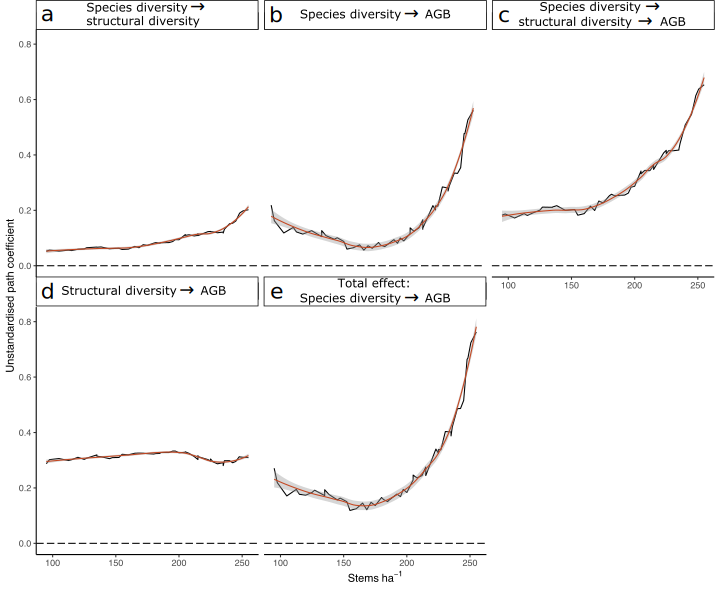
\includegraphics[width=0.8\textwidth]{sem_struc_stems_ha}
	\caption{Line charts showing the variation in path coefficients in the SEM, using datasets with different mean stem density.}
	\label{sem_struc_stems_ha}
\end{figure}

\subsection{Models with environmental covariates}

A model incorporating moisture availability and soil showed that at the regional level, the effect of diversity on biomass was greater than that of moisture and soil. Surprisingly, the effect of moisture availability on biomass was negligible, with all of the observed effect coming from the indirect path of moisture availability on biomass via species diversity. 

Soil fertility had a strong positive effect on species diversity. Soil fertility also had a positive effect on AGB.  

The effect of species diversity had the strongest total effect on biomass, with some indirect effect via structural diversity.

\begin{figure}[H]
\centering
	\includegraphics[width=\textwidth]{full_mod}
	\caption{Path diagram with regression coefficients for the full model incorporating environmental covariates and tree species diversity in all five clusters.}
	\label{full_mod}
\end{figure}

\begin{figure}[H]
\centering
	\includegraphics[width=\textwidth]{full_model_slopes}
	\caption{Standardized path coefficients for the interactive effects of abiotic environment and tree diversity on AGB across all plots. Path coefficients are +/- 1 standard error. Path coefficients where the standard error does not overlap zero are considered to be significant effects.}
	\label{full_model_slopes}
\end{figure}


% Table created by stargazer v.5.2.2 by Marek Hlavac, Harvard University. E-mail: hlavac at fas.harvard.edu
% Date and time: Tue, Oct 29, 2019 - 10:25:05
\begin{table}[!htbp] \centering 
  \caption{} 
  \label{full_model_fit_clust_stats} 
\begin{tabular}{@{\extracolsep{0pt}} ccccccccccc} 
\\[-1.8ex]\hline 
\hline \\[-1.8ex] 
{Cluster} & {Params.} & {n} & {$\chi^{2}$} & {DoF} & {CFI} & {TLI} & {LogLik} & {AIC} & {RMSEA} & {SRMR} \\
\hline \\[-1.8ex] 
C1 & 25 & 420 & 1259.430 & 53 & 0.460 & 0.327 & -6145.100 & 12340.200 & 0.230 & 0.187 \\ 
C2 & 25 & 671 & 1530.040 & 53 & 0.445 & 0.309 & -8588.900 & 17227.900 & 0.200 & 0.149 \\ 
C3 & 25 & 105 & 516.500 & 53 & 0.417 & 0.274 & -1055.300 & 2160.700 & 0.290 & 0.216 \\ 
C4 & 25 & 46 & 227.910 & 53 & 0.457 & 0.324 & -607.600 & 1265.200 & 0.270 & 0.233 \\ 
C5 & 25 & 84 & 489.700 & 53 & 0.387 & 0.237 & -1097.700 & 2245.400 & 0.310 & 0.328 \\ 
\hline \\[-1.8ex] 
\end{tabular} 
\end{table} 


\subsection{Structural diversity}

The latent variable of tree species diversity had a positive effect on AGB across the region. A stronger positive effect was seen between structural diversity and aboveground biomass, with species diversity acting \textit{through} structural diversity to effect aboveground biomass.

\subsection{Interaction effects of moisture availability and soil}

To further address our hypothesis (H\textsubscript{2}) that more arid plots and plots with less fertile soil will show a stronger positive effect of tree species richness on above ground woody biomass, we fit a separate model with the latent variables of moisture availability and soil fertility as moderators on the relationship between species diversity and AGB.

Moderating effects of moisture availability were not observed.

Soil fertility had a small positive effect on the relationship between species diversity and biomass. As soil fertility increased, the strength of the relationship between species diversity and biomass also increased. This effect was small in comparison to the direct effect of soil fertility on AGB.

\section{Discussion}

\bibliography{/Users/johngodlee/google_drive/bib/lib}

\subsection{Conclusion}


\end{document}

% Seidel 2019: Large trees tend to possess a greater structural complexity than small trees, not due to their size per se, but due to more complex architecture.

% https://jslefche.github.io/sem_book/coefficients.html

